\chapter{Complexité}
\section{Des exemples}

Voici trois exemples de problèmes qu'on peut vouloir résoudre 

\subsection{Test de primalité}
    Étant donné un entier $n$ plus grand que 1, cet entier est-il premier\footnote{\noindent est-ce qu'il existe d'autres diviseurs de $n$ que $1$ et $n$ ?} ou non ?\medskip

    Par exemple, 127 est-il premier ? Pour y répondre, on va diviser 127 par 2, par 3, par 4, \textit{et cætera}, et regarder si une de ces divisions « tombe juste » ou non. Si c'est le cas, 127 n'est pas premier. On n'a pas besoin de pousser les divisions jusqu'à 126, il suffit simplement d'aller jusqu'à $\lfloor\sqrt{127}\rfloor$, c'est-à-dire onze\footnote{\noindent en effet, si $n$ admet un diviseur, alors on peut écrire $n=pq$ avec $p$ et $q$ deux entiers et il y en a obligatoirement un des deux qui est plus petit ou égal à $\sqrt{n}$, donc à $\lfloor\sqrt{n}\rfloor$ puisqu'il est entier.}.\\
    Quand on le fait, on se rend compte que 127 est premier.

\subsection{Recherche de la présence d'un élément dans une liste}
    Étant donnée une liste d'entiers \mintinline{python}{lst} de longueur $n$ et un entier \mintinline{python}{val}, cet entier appartient-il ou non à \mintinline{python}{lst} ?\medskip

    Par exemple, avec une liste \mintinline{python}{lst} valant \mintinline{python}{[4, 2, 7, 8, 9]} et une valeur \mintinline{python}{val} de \mintinline{python}{5}, il faut parcourir \textit{intégralement} \mintinline{python}{lst} pour constater que \mintinline{python}{val} n'y figure pas.

\subsection{Table de multiplication}
    Étant donné un entier $n\in\N^*$, on veut afficher tous les nombres de la forme $i\times j$, avec $i$ et $j$ entiers compris entre 1 et $n$.\medskip

    Par exemple pour $n$ valant 4, j'obtiens la table suivante :
    \begin{center}
    \tabularstyled
    \begin{tabular}{c|c|c|c}
    1 & 2 & 3 & 4\\
    2 & 4 & 6 & 8 \\
    3 & 6 & 9 & 12 \\
    4 & 8 & 12 & 16            
    \end{tabular}
    \end{center}


Pour chacune des situations précédentes, $n$ est appelé \textit{taille du problème}. Plus $n$ augmente, plus le nombre d'opérations (au sens large : calculs, tests, accès aux éléments d'une liste, \textit{et cætera}) augmente.\\

À quelle vitesse ce nombre d'opérations augmente-t-il ?\\

S'il y a plusieurs algorithmes pour résoudre un même problème, y en a-t-il un plus efficace que les autres, c'est-à-dire dont le nombre d'opérations augmente moins vite lorsque $n$ augmente ?

\section{Complexité temporelle}

Évaluer la complexité temporelle d'un algorithme, c'est estimer le nombre d'opérations \textit{significatives} qui entrent en jeu lors de la résolution par cet algorithme d'un problème de taille $n$. 

\begin{methode}[ : évaluation de la complexité temporelle]
Pour évaluer l'efficacité d'un algorithme en terme de nombre d'opérations
\begin{itemize}
   \item    d'abord on décide ce qu'est une opération significative. On appelle ceci une \textsc{opel} ; 
   \item    seules les \textsc{opel} sont considérées comme coûteuses en temps et sont comptabilisées ;
   \item    les autres opérations sont \textit{négligées} ;
   \item    on cherche à estimer le nombre d'\textsc{opel} nécessaires à la résolution par l'algorithme d'un problème de taille $n$. 
\end{itemize}
\end{methode}                                   


On peut « imaginer » une fonction $c_M$ (au sens mathématique du terme) qui serait définie pour toute taille $n$ du problème et	donnerait le nombre \textit{moyen}  d'\textsc{opel} nécessaires pour résoudre un problème de taille $n$.\\
Cette \textit{complexité moyenne} est très rarement calculable car les calculs trop compliqués.\\


Plus simple mais tout aussi utile que $c_M$, est la complexité \textit{dans le pire des cas}.

\begin{definition}[ : complexité dans le pire des cas]
Pour un problème de taille $n$, on note $c(n)$ le nombre maximal d'\textsc{opel} pour résoudre un problème de cette taille.
\end{definition}

En pratique, on ne calcule pas \textit{exactement} $c(n)$. On se contente d'indiquer à quelle vitesse $c(n)$ augmente lorsque $n$ augmente, en se servant de \textit{fonctions de référence} telles que celles représentées ci-dessous.\\

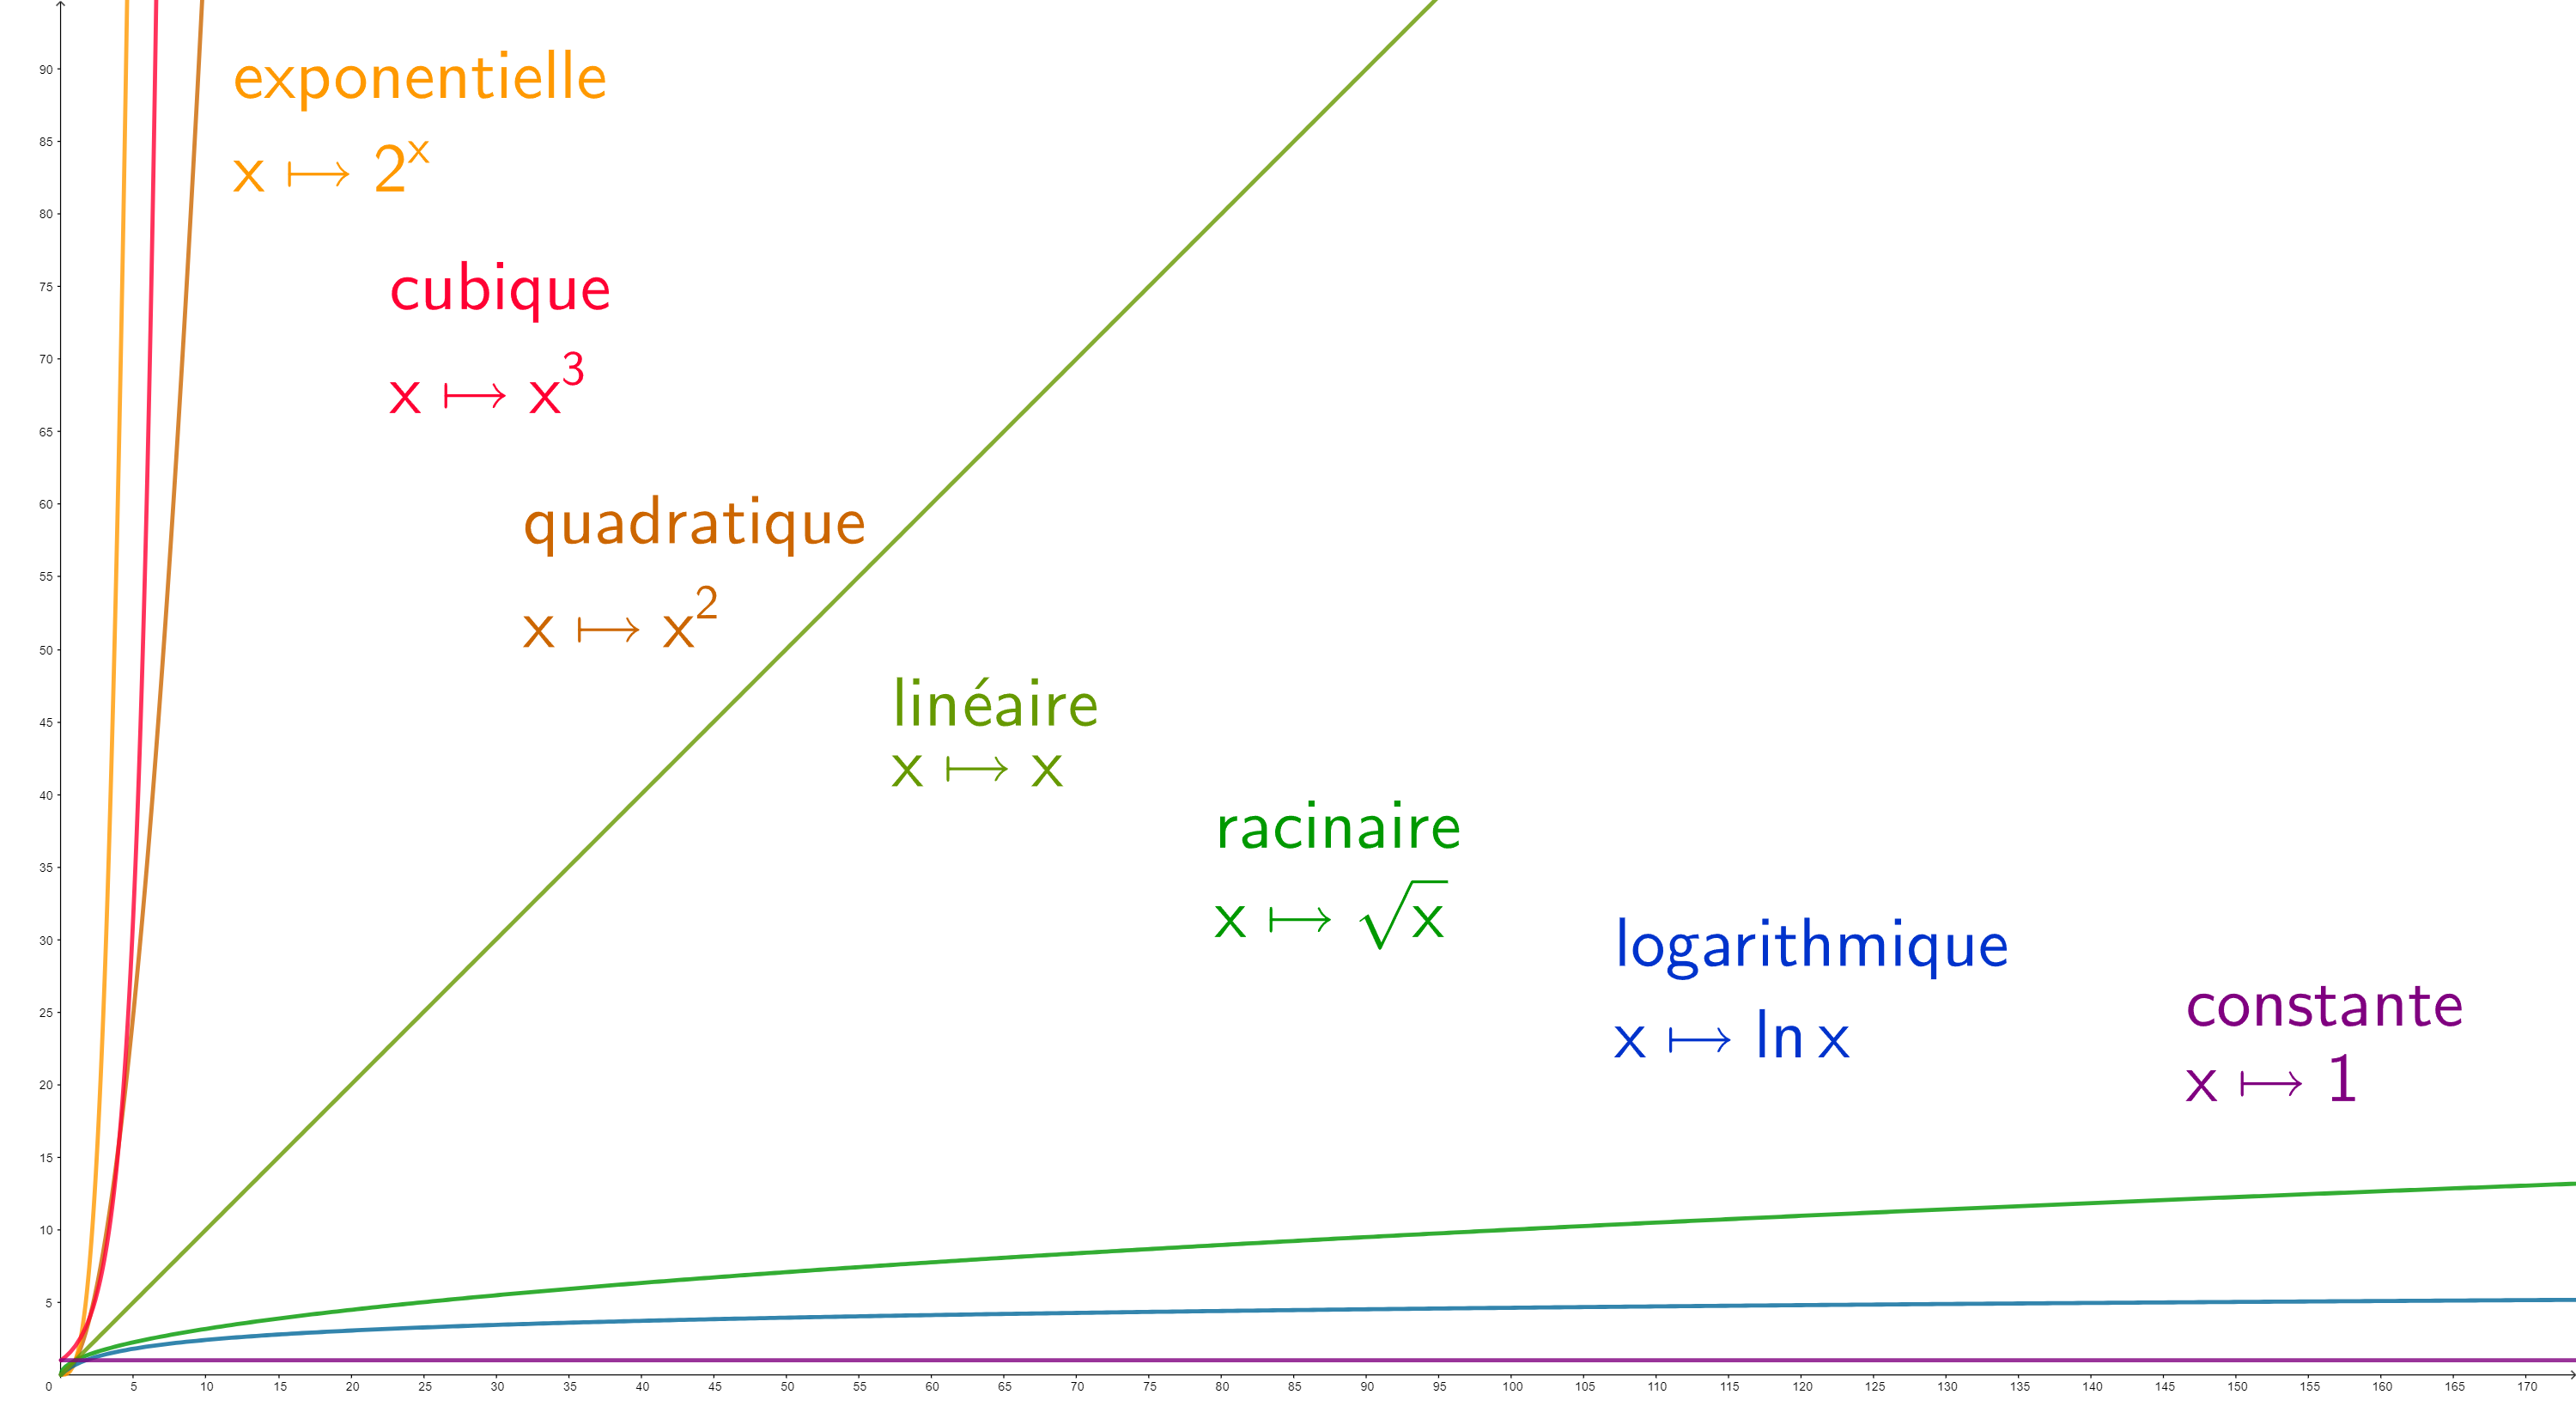
\includegraphics[width=\linewidth]{ch-complexite/img/complexite}

Il est très utile de connaître la complexité d'un algorithme car cela nous permet d'estimer le temps de resolution d'un problème quand on connaît l'ordre de grandeur de $n$ comme le montre le tableau ci-dessous.
\begin{center}

\tabularstyled
\renewcommand{\arraystretch}{1.5}
\scriptsize
\begin{tabular}{c|c|c|c|c|c|c|c|c}
\rowcolor{UGLiOrange}
& {\ths5} & {\ths10} & {\ths20} & {\ths50} & {\ths250} & {\ths1 000} & {\ths10 000} & {\ths1 000 000} \\
constante & 10 ns & 10 ns & 10 ns & 10 ns & 10 ns & 10 ns & 10 ns & 10 ns \\
logarithmique & 10 ns & 10 ns & 10 ns & 20 ns  & 30 ns & 30 ns & 40 ns & 60 ns \\
racinaire & 22 ns & 32 ns & 45 ns & 71 ns & 158 ns & 316 ns & 1 µs & 10 µs \\
linéaire & 50 ns & 100 ns & 200 ns & 500 ns & 2,5 µs & 10 µs & 100 µs & 10 ms \\
quadratique & 250 ns & 1 µs & 4 µs & 25 µs & 625 µs & 10 ms & 1 s & 2,8 h \\
cubique & 1,25 µs & 10 µs & 80 µs & 1.25 ms & 156 ms & 10 s & 2,7 h & 316 ans \\
exponentielle & 320 ns & 10 µs & 10 ms & 130 jours & $10^{59}$ ans & \ldots & \ldots & \ldots \\
\end{tabular}
\renewcommand{\arraystretch}{1}
\end{center}


\section{Application à nos exemples}

\subsection{Test de primalité}

\begin{pyc}
   \begin{minted}{python}
      from math import sqrt
      def est_premier(n: int) -> bool:
         # on parcourt les entiers de 2 à racine(n)
         for i in range(2, int(sqrt(n)) + 1):
            # si une division tombe juste
            if n % i == 0:
               # alors n n'est pas premier
               return False
         # si aucune ne tombe juste il est premier
         return True
   \end{minted}
\end{pyc}

On convient qu'une \textsc{opel} est une division. Pour $n$ fixé, on effectue au pire des cas les divisions par 2, 3, \ldots, $\lfloor\sqrt{n}\rfloor$, il y en a \textit{grosso modo} $\sqrt{n}$ : notre algorithme est de complexité racinaire\footnote{en réalité c'est sans doute plus que cela car plus $n$ est grand, plus les nombres qui entrent en jeu dans les divisions sont grands et plus les divisions prennent de temps.}. 

\subsection{Recherche de la présence d'un élément dans une liste}

\begin{pyc}
   \begin{minted}{python}
      def present(lst: list, val: int) -> bool:
         # on parcourt la liste par ses éléments
         for x in lst:
            # si on trouve val
            if x == val:
               # on renvoie True
               return True
         # si on ne l'a pas trouvé, on renvoie False
         return False
   \end{minted}
\end{pyc}
Ici une \textsc{opel} sera un accès à un élément de la liste, c'est à dire le fait d'attribuer les valeurs à la variable \mintinline{python}{x}. Pour une liste de taille $n$ fixé, dans le pire des cas \mintinline{python}{val} n'appartient pas à \mintinline{python}{lst} et on effectue $n$ \textsc{opel} : notre algorithme est de complexité linéaire.

\subsection{Table de multiplication} 

\begin{pyc}
   \begin{minted}{python}
      def affiche(n: int) -> None:
         for i in range(1, n + 1):
            for j in range(1, n + 1):
               print(i * j)
   \end{minted}
\end{pyc}

Ici une \textsc{opel} est une multiplication. Pour $n$ fixé, dans tous les cas on effectue deux boucles imbriquées, donc $n\times n$ sont effectuées et notre algorithme est de complexité quadratique.

\section{Exercices}
\begin{exercice}
   Une \textsc{opel} est une addition, déterminer la complexité de la fonction suivante:
   \begin{minted}{python}
   def somme(n: int) -> int:
      s = 0
      for i in range(1, n + 1):
         s += i
      return s
    \end{minted} 
\end{exercice}

\begin{exercice}[ : nombre de bits d'un entier]
   La fonction suivante 
   \begin{itemize}
      \item prend en entrée un \mintinline{python}{n} non nul ;
      \item renvoie le nombre de bits nécessaires à l'écriture de $n$ en base 2. 
   \end{itemize}
   
   \begin{minted}{python}
   def nb_bits(n: int) -> int:
   b = 0
   while n > 0:
      b += 1
      n = n // 2
   return b
   \end{minted}
   Une \textsc{opel} est une division par 2. En testant la fonction \mintinline{python}{nb_bits} sur des entiers de plus en plus grands, conjecturer la complexité de cette fonction. 

\end{exercice}

\begin{exercice}[* : addition de matrices]
   On considère des \textit{matrices}, qui sont représentées par des listes de listes d'\mintinline{python}{int} ($n$ lignes et $n$ colonnes).
   Par exemple les matrices 
   \tabulardefault
   $$M_1 = \begin{matrice}
         1 & 2 & -1\\
         0 & -1 & 2\\
         -1& 1 & 0\\
   \end{matrice}\quad\text{et}\quad M_2 = \begin{matrice}
         -3 & 1 & 0\\
         1 & 0 & -2\\
         1& -1 & 1\\
   \end{matrice}$$
   sont deux matrices carrées d'ordre 3 et sont représentées en \textsc{Python} par \\
   \mintinline{python}{m1 = [[1, 2, -1], [0, -1, 2], [-1, 1, 0]]} et\\
   \mintinline{python}{m2 = [[-3, 1, 0], [1, 0, -2], [1, -1, 1]]}\\

   Il est possible d'ajouter 2 matrices de même taille en procédant « case par case »  :
   $$M_1+M_2 = \begin{matrice}
         -2 & 3 & -1\\
         1 & -1 & 0\\
         0& 0 & 1\\
   \end{matrice}$$
   En convenant qu'une \textsc{opel} est une addition de deux \mintinline{python}{int} , sans écrire l'algorithme, donner la complexité de l'algorithme d'addition de deux matrices.
\end{exercice}
\begin{exercice}[* : multiplication de matrices]
   Il est possible de multiplier 2 matrices de même taille suivant l'algorithme suivant :
  
      \begin{minted}{python}
         def produit(m1: list, m2: list) -> list:
            # n est la taille des matrices
            n = len(m1) 
            # on crée une matrice remplie de zéros
            p = [[0 for j in range(n)] for i in range(n)]
            # pour chaque ligne
            for i in range(n):
               # pour chaque colonne
               for j in range(n):
                  # on ajoute tous ces nombres
                  for k in range(n):
                     p[i][j] += m1[i][k] * m2[k][j]
            # puis on renvoie la matrice produit
            return p
      \end{minted}


   Déterminer la complexité de cet algorithme.
\end{exercice}
